\paragraph{}
In this example, a plane strain bracket with a downward uniform distributed load on the top is considered (see Fig.~\ref{adp_fig:ex_bracket_geo_bc}).
The material properties are: Young’s modulus $E = \SI{2e5}{\newton \per \square \meter}$ and Poisson’s ratio $\nu = 0.3$.
    \begin{figure}
        \centering
        \begin{subfigure}[b]{1\linewidth}
            \centering
            \scalebox{1.2}{
                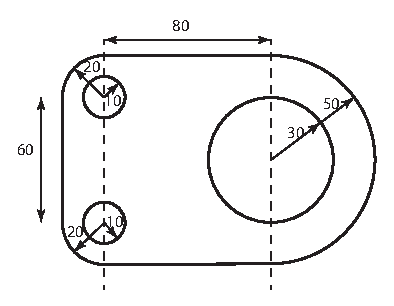
\includegraphics{quadtree/ex_images/ex_bracket_geo.eps}
            }
        \end{subfigure}
    \end{figure}
    \begin{figure}\ContinuedFloat
        \begin{subfigure}[b]{1\linewidth}
            \centering
            \scalebox{1.3}{
                
\includegraphics{quadtree/ex_images/ex_bracket_load.eps}
            }
        \end{subfigure}
        \caption{ Plane strain bracket: geometry and boundary conditions}
        \label{adp_fig:ex_bracket_geo_bc}
    \end{figure}

\paragraph{}
A total strain energy of $\SI{282.927}{\joule}$ is determined by ANSYS with the mesh shown in Fig.~\ref{qdt_fig:ex_bracket_ansys_mesh}

% /* cSpell:disable */
% -1 - 282.927
% 382*2  - 274.5638 (32-4/8-3)
% 950*2  - 280.1255 (64-4/8-3)
% 2110*2 - 281.0799 (128-4/15-4)
% 4414*2 - 282.0363 (256-4/15-4)


% mlp
% 530 - 279.8076
% 1554 - 282.0745
% 4208 - 282.5681
% err = abs([279.8076 ,282.0745,282.5681]-282.927)/282.927; dof = [530,1554,4208]; polyfit(log(dof),log(err),1)

% uniform
% 530 - 279.8076
% 1810 - 282.3186
% 6464 - 282.674
% err_un = abs([279.8076 ,282.3186 ,282.674]-282.927)/282.927; dof_un = [530,1810,6464]; polyfit(log(dof_un),log(err_un),1)

% ansys-2nd
% 406*2 -  282.412
% 1144*2 - 282.895
% 4270*2 - 282.923

% 16462*2 -  282.926
% err_a2 = abs([282.412,282.895,282.923]-282.927)/282.927; dof_a2 = [406,1144,4270]*2; polyfit(log(dof_a2),log(err_a2),1)

% ansys-1st
% 185*2 - 275.635    
% 650*2 -  280.006   
% 1227*2 -  281.502 
% 2405*2 - 282.136
% err_a1 = abs([275.635,280.006  ,281.502 ,282.136]-282.927)/282.927; dof_a1 = [185,650,1227,2405]*2; polyfit(log(dof_a1),log(err_a1),1)

% disp > 0.01
% 530 - 279.8076
% 1348 - 281.4530
% 2768 - 282
% 5438 - 282.2
% err_d = abs([279.8076, 281.4530  ,282 ,282.2]-282.927)/282.927; dof_d = [530,1348,2768,5438]; polyfit(log(dof_d),log(err_d),1)

% str > 0.1
% 530 - 279.8076
% 1514 - 281.8970
% 4336 - 282.1295

% err_s = abs([279.8076, 281.8970  ,282.1295 ]-282.927)/282.927; dof_s = [530,1514,4336]; polyfit(log(dof_s),log(err_s),1)


% /* cSpell:enable */
\paragraph{}
% result analysis
The rate of convergence in terms of the total strain energy is shown in Fig.~\ref{adap_fig:ex_bracket_conv} and corresponding mesh development are presented in Fig.~\ref{adap_fig:ex_bracket_mesh_sbfem} (SBFEM) and Fig.~\ref{adap_fig:ex_bracket_mesh_ansys} ( Ansys 4-node quadrilateral element ).
Higher convergence rate compared to the result determined in ANSYS is observed.

\begin{figure}[h!]
    \centering
    \scalebox{0.5}{
        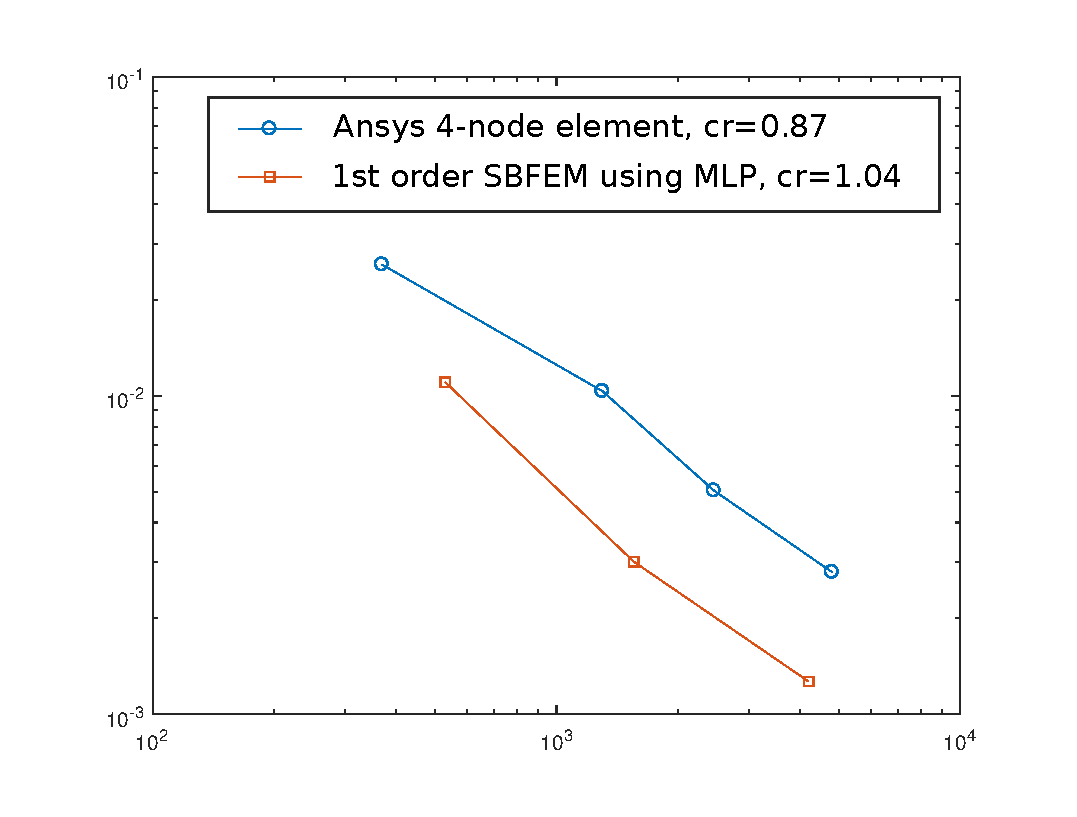
\includegraphics{adaptivity/ex_images/ex_adap_bracket_conv.eps}
    }
    \caption{Plane strain bracket: Convergence study}
    \label{adap_fig:ex_bracket_conv}
\end{figure}

\begin{figure}[h!]
    \centering
    \begin{subfigure}[b]{0.4\linewidth}
        \centering
        \scalebox{0.6}{
            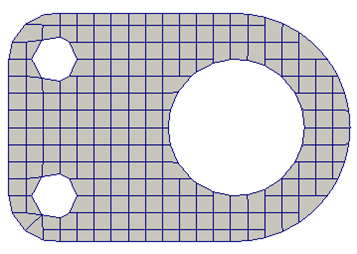
\includegraphics{adaptivity/ex_images/ex_adap_bracket_530.png}
        }
        \caption{Initial mesh, 530 DOFs}
    \end{subfigure}
    \begin{subfigure}[b]{0.4\linewidth}
        \centering
        \scalebox{0.6}{
            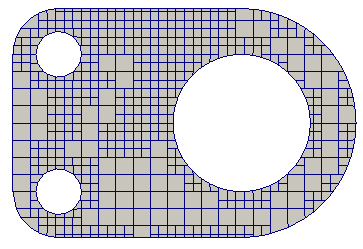
\includegraphics{adaptivity/ex_images/ex_adap_bracket_1554.png}
        }
        \caption{1st refinement, 1554 DOFs}
    \end{subfigure} \\
    \begin{subfigure}[b]{1\linewidth}
        \centering
        \scalebox{0.8}{
            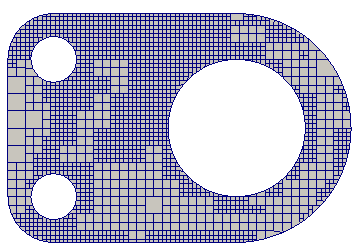
\includegraphics{adaptivity/ex_images/ex_adap_bracket_4208.png}
        }
        \caption{2nd refinement, 4208 DOFs}
    \end{subfigure}
    \caption{Plane strain bracket: Mesh development (SBFEM)}
    \label{adap_fig:ex_bracket_mesh_sbfem}
\end{figure}


\begin{figure}[h!]
    \centering
    \begin{subfigure}[b]{0.48\linewidth}
        \centering
        \scalebox{0.4}{
            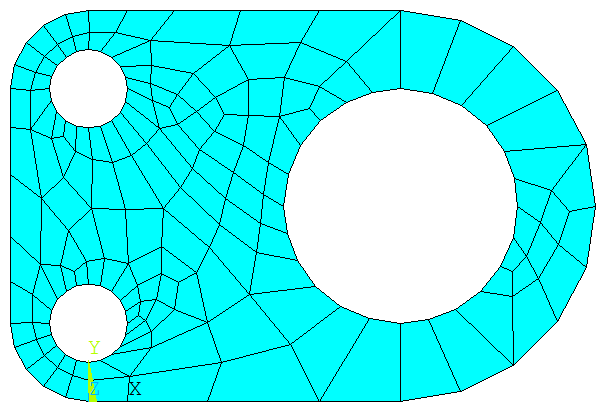
\includegraphics{adaptivity/ex_images/ex_adp_bracket_ansys_185.png}
        }
        \caption{Initial mesh, 138 DOFs}
    \end{subfigure}
    \begin{subfigure}[b]{0.48\linewidth}
        \centering
        \scalebox{0.4}{
            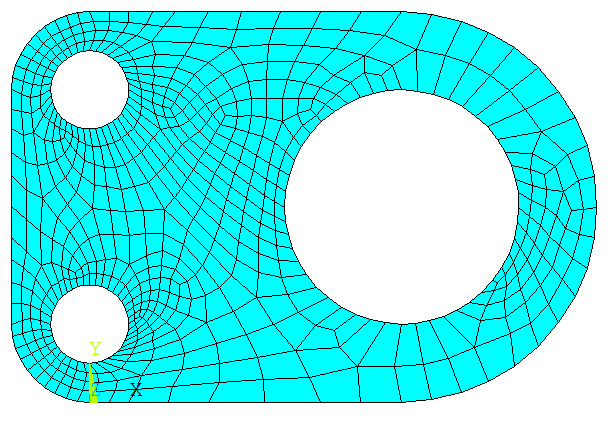
\includegraphics{adaptivity/ex_images/ex_adp_bracket_ansys_650.png}
        }
        \caption{1st refinement, 482 DOFs}
    \end{subfigure}
    \begin{subfigure}[b]{0.48\linewidth}
        \centering
        \scalebox{0.4}{
            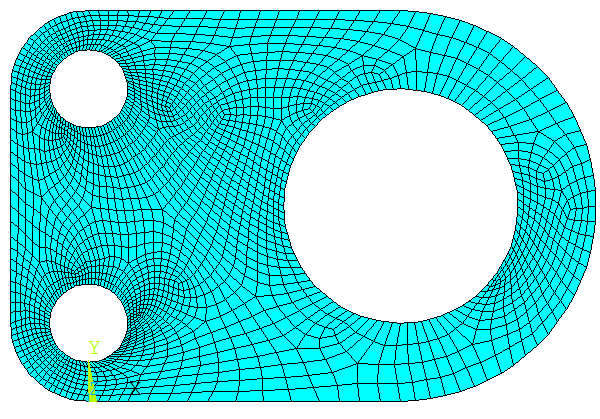
\includegraphics{adaptivity/ex_images/ex_adp_bracket_ansys_1227.png}
        }
        \caption{2nd refinement, 1794 DOFs}
    \end{subfigure}
    \begin{subfigure}[b]{0.48\linewidth}
        \centering
        \scalebox{0.4}{
            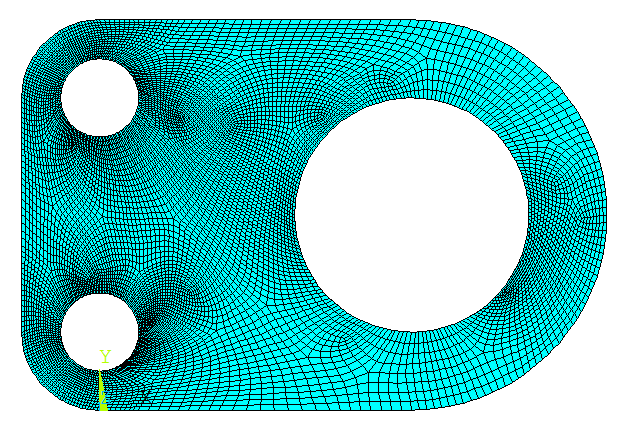
\includegraphics{adaptivity/ex_images/ex_adp_bracket_ansys_2405.png}
        }
        \caption{3rd refinement, 6914 DOFs}
    \end{subfigure}
    \caption{Plane strain bracket: Mesh development (Ansys)}
    \label{adap_fig:ex_bracket_mesh_ansys}
\end{figure}
